\chapter{Método de trabajo}
\label{chap:metodo}
\drop{T}ras haber analizado cuales son los objetivos a desarrollar en el TFG, y realizado un análisis de las tecnologías existentes, es necesario asignar una metodología para la gestión del proyecto. 

Para ello, y valorando el número de personas que están involucradas en el proyecto (director del TFG y su autor), se realiza una investigación sobre cuales son las alternativas de metodologías para llevarlo a cabo, que sea ágil, ligera, y por supuesto, flexible a cambios para adaptar nuevos requisitos que puedan surgir.

Las metodologías Agile, surgen en el año 1990, como herramienta de gestión software que indicase unas correctas directivas para llevar a acabo los proyectos. 

Las metodologías existentes hasta la época, tenían una rigurosa asignación de roles, actividades y artefactos (incluyendo el modelado y una documentación muy detallada), que no obstante, a día de hoy sigue siendo necesaria para proyectos de gran envergadura, que necesitan una alta gestión de tiempo y recursos. 

Según avanza el desarrollo de aplicaciones software, entran en escena nuevas situaciones en las cueles este tipo de métodos de gestión no encaja totalmente con estas metodologías tradicionales. 

Los métodos Agile promueven una gestión de proyectos, que se basa principalmente en fomentar la constante inspección del trabajo y la adaptación de éste. Se trata de un sistema organizado que facilita el trabajo el equipo, una correcta organización, y favorece el rendimiento del tiempo empleado en el desarrollo.

Scrum fue creado, con las características de estos métodos de gestión, trabajando con una comunicación directa y empleando ingeniería concurrente, basándose en las ideas del «Manifiesto por el Desarrollo Ágil de Software» (detalladas en la siguiente sección del documento).

Por lo tanto, basándose en estas ideas, y teniendo en cuenta el número de personas que están involucradas en el proyecto, se ha elegido la metodología de trabajo Scrum.


\section{Metodología Agile}



\section{Scrum como metodología de trabajo}



\subsection{Roles}



\subsection{Artefactos}



\subsection{Motivos de la elección del método Scrum}



\section{Aplicación del método de trabajo}

\subsection{Iteración : Sistema de localización del Widget tangible sobre la pantalla táctil}
Uno de los objetivos principales de este TFG es diseñar y programar un sistema de localización y reconocimiento entre las dos interfaces de usuario tangibles. Este sistema de localización consiste en obtener las coordenadas de la posición del «Widget tangible» (TUIO2[MANDAR A ENLACE]) sobre la pantalla táctil capacitiva del dispositivo TUIO1[MANDAR A ENLACE]. Estas coordenadas son enviadas desde TUIO1 a TUIO2. Lo que se quiere obtener es una representación en la pantalla de TUIO2 de la imagen o animación de lo que muestra la pantalla de TUIO1.\\
Antes de posicionar TUIO2 sobre TUIO1, las pantallas de ambos dispositivos muestran imágenes diferentes (ver Figura~\ref{fig:Localizacion1}).
\begin{figure}[!h]
\begin{center}
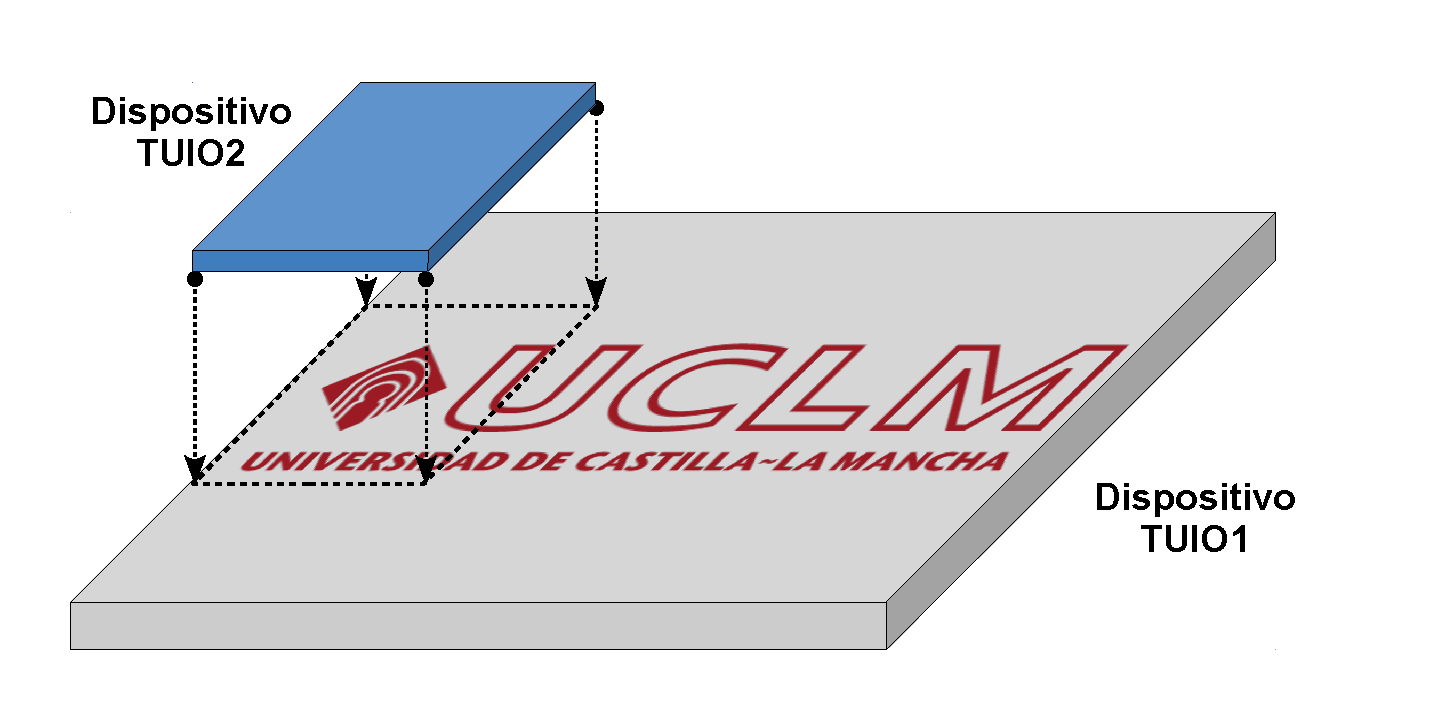
\includegraphics[width=0.7\textwidth]{localizacion1.pdf}
\caption{Posición de los dispositivos antes de la interacción sobre la pantalla capacitiva}
\label{fig:Localizacion1}
\end{center}
\end{figure}
Al posicionar TUIO2 sobre la pantalla de TUIO1, la pantalla de TUIO2 muestra la parte de imagen correspondiente que es tapada por el dispositivo como se muestra en la Figura~\ref{fig:Localizacion2}:
\begin{figure}[!h]
\begin{center}
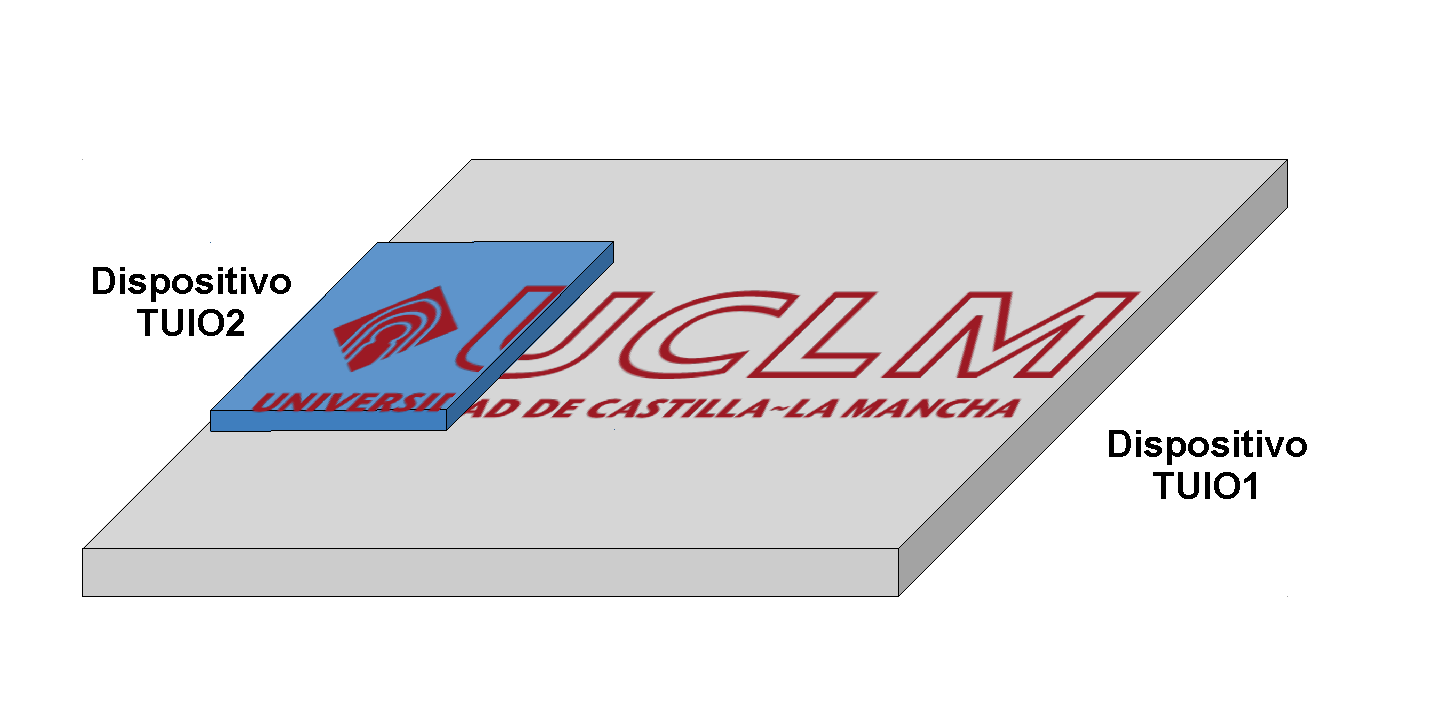
\includegraphics[width=0.7\textwidth]{localizacion2.pdf}
\caption{Posición de los dispositivos despues de la interacción sobre la pantalla capacitiva}
\label{fig:Localizacion2}
\end{center}
\end{figure}


\subsubsection{Localización del Widget tangible TUIO2}

El procedimiento para obtener la posición de del dispositivo TUIO2 sobre la pantalla del dispositivo TUIO1, se consigue mediante el uso del sensor capacitivo de la propia pantalla de TUIO1, que al detectar una variación de la capacitancia genera un evento táctil.
El dispositivo TUIO2 produce tres eventos táctiles sobre la pantalla capacitiva. Estos eventos son generados por medio de tres almohadillas de goma conductora que están conectadas al borne negativo de la «RaspberryPi». Esta conexión evita que el usuario tenga que sostener con su propia mano el dispositivo, haciendo de conexión a tierra el propio borne negativo.
El diseño de los puntos de contacto es el que se muestra en la siguiente Figura~\ref{fig:Localizacion3}.
\begin{figure}[!h]
\begin{center}
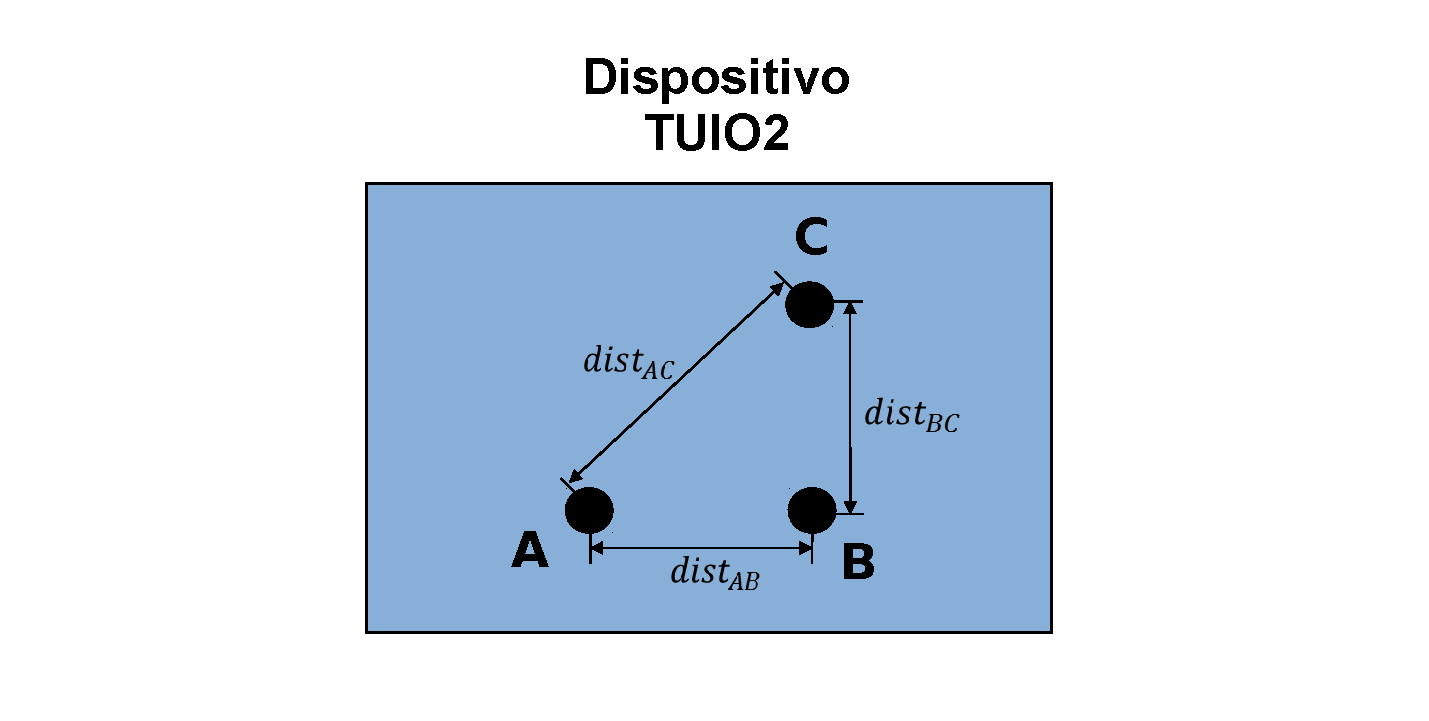
\includegraphics[width=0.9\textwidth]{localizacion3.pdf}
\caption{Disposición de las almohadillas conductoras en la parte inferior del «Widget tangible» para generar los eventos táctiles. }
\label{fig:Localizacion3}
\end{center}
\end{figure}
Los tres puntos de contacto son identificados A, B y C, que dan nombre a los vértices del triángulo rectángulo escaleno que forman. Se ha elegido este tipo de diseño ya que cada uno de los tres lados tiene una medida diferente, lo que hace que sea mas fácil identificar cada segmento del triangulo y así evitar posibles problemas cuando se localice cualquiera de sus vértices.

Cuando TUIO2 está sobre la pantalla, los eventos táctiles generados proporcionan la siguiente información al dispositivo TUIO1: posición e ID del evento. Las coordenadas de la posición de cada evento táctil es medida en pixels, por lo que cada evento producido será manejado en esas unidades de media (ver Figura~\ref{fig:Localizacion4}).\\
\begin{figure}[!h]
\begin{center}
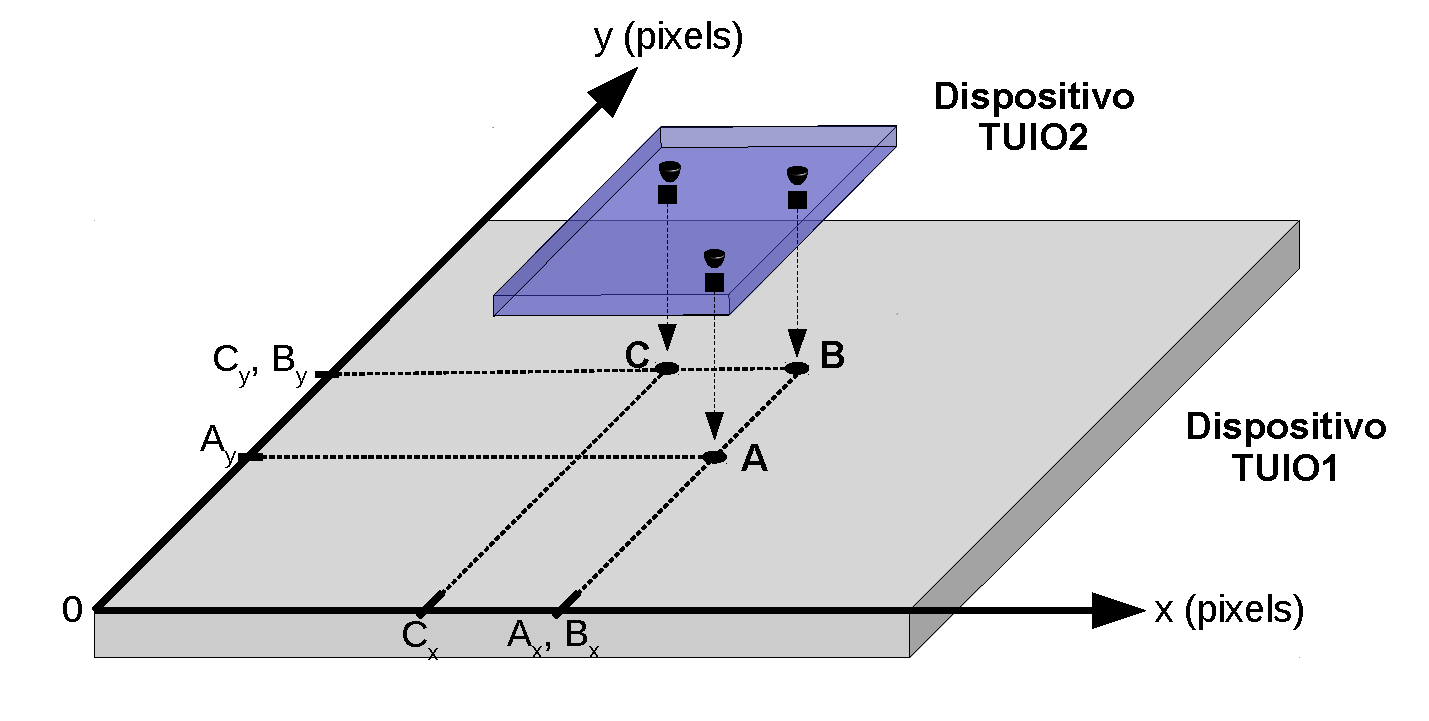
\includegraphics[width=0.9\textwidth]{localizacion4.pdf}
\caption{Coordenadas de los puntos A, B y C del «Widget tangible» sobre la pantalla capacitiva. }
\label{fig:Localizacion4}
\end{center}
\end{figure}
Estos datos son interpretados y tratados para calcular la posición de TUIO2 mediante un programa en «Python».

\subsubsection{Programa para la localización.}

Todos los eventos táctiles generados sobre la pantalla capacitiva del dispositivo TUIO1 son manejados por la \textit{clase Widget} en «Kivy», mediante el método \texttt{on\_touch\_down().}\\
Este método obtiene la información de posición e ID del evento táctil producido, almacenando estos datos en la lista \texttt{touch[].}\\
Se crea una librería específica para el manejo de esta lista, la cual se tratará y manejara los datos para obtener la información de posición de TUIO2.

\textbf{Método \texttt{pulsacion(touch)}}\\
El argumento de entrada corresponde con las coordenadas y la id del evento táctil que contiene la lista de eventos (\texttt{touch}).\\
Estos datos son almacenados en la última posición de la lista \texttt{puls[]} mediante el método \texttt{append()}:\\
\texttt{self.puls.append((t.x,t.y,t.id))}.\\
donde: \\
\texttt{t.x}: coordenada x del evento táctil.\\
\texttt{t.y}: coordenada y del evento táctil.\\
\texttt{t.id}: identificación del evento táctil (número de evento).\\
Cuando el número de eventos almacenados en \texttt{puls[]}   
es mayor que 1, se llama al método \texttt{determinar\_distancias()}.

\textbf{Método \texttt{determinar\_distancias()}}.\\
Mediante el método \texttt{Vector()}, de la librería \texttt{kivy}, es determinada la distancia entre los eventos táctiles producidos hasta el momento, y que son almacenados en la lista \texttt{puls[]}, haciendo uso de un bucle el cual recorre desde el último elemento de la lista \texttt{puls[]} hasta el primero. El método \texttt{determinar\_lados} es llamado en cada medida que se realiza de la distancia. Si la distancia es correcta, se incrementa la variable \texttt{contador}, la cual al llegar a 2, llama al método \texttt{determinar\_puntos()}.

\textbf{Método \texttt{determinar\_lados()}}.\\
Método para verificar si los dos eventos táctiles de los cuales se han determinado la distancia, corresponden con uno de los lados del triángulo del \textit{Widget tangible}, donde \textit{m} corresponde con la distancia entre los dos eventos táctiles, \textit{i} el tamaño de la lista \texttt{puls[]}, y \textit{a} el número de iteración del bucle que recorre cada uno de los elementos de la lista \texttt{puls[]}.

Este método es llamado cada vez que el método \texttt{determinar\_distancias()} es invocado.
Se comprueba si la distancia entre los dos puntos corresponde con el rango de medidas establecidos para los lados del triangulo del \emph{Widget tangible}. Los rangos de medida son los mostrados en la siguiente tabla (~\ref{tab:intervalos-coordenadas}).

\begin{table}[hp]
  \centering
  {\small
  


\begin{tabular}{p{.2\textwidth}p{.2\textwidth}}
  \tabheadformat
  \tabhead{Rango}   &
  \tabhead{Segmento del triángulo}  \\
\hline
(120,150) & AB \\
\hline
(160,150) & BC \\
\hline
(210,260) & AC
\end{tabular}


% Local variables:
%   coding: utf-8
%   ispell-local-dictionary: "castellano8"
%   TeX-master: "main.tex"
% End:

  }
  \caption[Intervalos de medida de cada segmento del triángulo]
  {Intervalos de medida de cada segmento del triángulo}
  \label{tab:intervalos-coordenadas}
\end{table}
Si la medida corresponde con alguno de los rangos establecidos, dicha medida es almacenada junto con las coordenadas de ambos eventos en la lista \texttt{dist[]}. Por ejemplo si la distancia entre los dos eventos táctiles es correcta y corresponde al segmento AB, los datos en la lista \texttt{dist[]} son almacenados de la siguiente manera:\\
\texttt{self.dist.append((m,'AB',toq1,toq2)) }\\
donde \texttt{m} corresponde a la distancia entre ambos puntos, \texttt{AB} es el nombre del segmento al que corresponde, \texttt{toq1} son las coordenadas del evento táctil con el cual se está midiendo la distancia en el método \texttt{determinar\_distancias()}, y \texttt{toq2} son las coordenadas del ultimo evento táctil.
Si la distancia es correcta se incrementa en una unidad la variable \texttt{contador}.

\textbf{Método \texttt{determinar\_puntos()}}.\\
Este método es invocado dentro del método \texttt{determinar\_distancias()} cuando la variable \texttt{contador} es mayor a 1, es decir, existen dos segmentos correctos del triángulo cuyos datos han sido almacenados en la lista \texttt{dist[]}, la cual contiene en ese momento dos elementos.
Los puntos del triangulo (A,B,C), son determinados siguiendo la siguiente lógica:
Por ejemplo, si los segmentos de los elementos de \texttt{dist[]} corresponden con $\overline{BC}$ y  $\overline{AB}$ respectivamente, se llama al método \texttt{asignar\_puntos}, donde los argumentos de entrada se establecen de la manera que sigue:

\texttt{self.asignar\_puntos(1,2,0,'B','C','A')}\\

A continuación se procede a detallar el método \texttt{asignar\_puntos}.

\textbf{Método \texttt{asignar\_puntos()}}.\\
Mediante este método se asigna a cada vértice A, B y C del triángulo, las coordenadas donde se encuentra cada uno de ellos, al igual que el nombre del vertice, y se almacenan dichos datos en la lista \texttt{coordenadas[]}

Para establecer un orden a la hora de añadir los valores a la lista \texttt{coordenadas[]} se pasa como argumentos la posición a la que corresponden cada uno de los puntos.\\
0: corresponde a la posición de la letra A en la lista \texttt{coordenadas[].}\\
1: posición de la letra B para la lista \texttt{coordenadas[]}.\\
2: posición de la letra C en la lista \texttt{coordenadas[]}.\\

La finalidad es que la lista \texttt{coordenadas} quede con la siguiente estructura para ser 
manejada:\\

$[(x_{A},y_{A},'A'),(x_{B},y_{B},'B'),(x_{C},y_{C},'C')]$\\

En el ejemplo anterior teniamos que los elementos de \texttt{dist[]} corresponden con $\overline{BC}$ y $\overline{AB}$. El punto en común para ambos segmentos corresponde a \textit{\textit{B}}, \textit{C} para el primer segmento, y \textit{A} para el segundo segmento
La llamada al método para asignar los puntos es:\\
\texttt{self.asignar\_puntos(1,2,0,'B','C','A')}\\
donde los argumentos de entrada son:
c = 1, posición del punto en común entre los dos segmentos. Como el punto en comun es \textit{B} que corresponde con la posición 1 de la lista \texttt{coordenadas[]}.\\
c1 = 2, es la posición del punto \textit{C} para el ejemplo, según el criterio establecido.\\
c2 = 0, corresponde a la posición del punto \textit{A} para la lista \texttt{coordenadas[]}.\\
p = 'B', Nombre del vértice en común, en este ejemplo corresponde al vértice \textit{B}.\\
p1 = 'C', Nombre del vértice restante del primer segmento, en este caso el primer segmento es el $\overline{BC}$, por lo tanto el vértice corresponde al \textit{C}.\\
p2 = 'A', Nombre del vértice del segundo segmento, que corresponde con el vértice \textit{A}.\\

Siguiendo con el ejemplo, los valores que contiene la lista \texttt{dist[]} para ser manejados por el método \texttt{asignar\_puntos()} son:
\texttt{[(0, 'NADA'), (164.0, 'BC', (440.00000000000006, 346.0, 'mouse2'), (440.00000000000006, 182.0, 'mouse1')), (134.03357788255903, 'AB', (306.0, 179.0, 'mouse3'), (440.00000000000006, 182.0, 'mouse1'))]}\\

La lista es recorrida mediante el siguiente bucle (ver Listado~\ref{code:buclevertices}):
\begin{lstlisting}[
  float    = ht,  
  language = python,
  caption  = {«Bucle para asignar las coordenadas de los vértices»},
  label    = code:buclevertices]
for a in r
	for b in range(2):
		if self.dist[1][a+2][2] == self.dist[2][b+2][2]:
			self.coordenadas[c] = (self.dist[1][a+2][0],self.dist[1][a+2][1],p)
			if a == 0:
				self.coordenadas[c1] = (self.dist[1][3][0],self.dist[1][3][1],p1)
			else:
				self.coordenadas[c1] = (self.dist[1][2][0],self.dist[1][2][1],p1)
			if b == 0:
				self.coordenadas[c2] = (self.dist[2][3][0],self.dist[2][3][1],p2)
			else:
				self.coordenadas[c2] = (self.dist[2][2][0],self.dist[2][2][1],p2)
			break
\end{lstlisting}
Donde \texttt{a} es la posición para el primer elemento de la lista \texttt{dist[]}, y \texttt{b} la posición del segundo elemento de la lista \texttt{dist[]}

El bucle busca cuales son las coordenadas en común entre los dos segmentos del triangulo. La lista \texttt{dist[]} contiene dos elementos que son los dos segmentos del triangulo con las coordenadas de los eventos táctiles, por lo tanto se recorre las coordenadas de los segmentos buscando la \textit{id} en común. 

Para poder analizar mejor este ejemplo, separamos los dos elementos de la lista \texttt{dist[]}:\\

\texttt{Elemento 1 de dist[]}:\\
\texttt{(164.0, 'BC', (440.00000000000006, 346.0, 'mouse2'), (440.00000000000006, 182.0, 'mouse1'))}\\

\texttt{Elemento 2 de dist[]}:\\
\texttt{(134.03357788255903, 'AB', (306.0, 179.0, 'mouse3'), (440.00000000000006, 182.0, 'mouse1'))}\\

La \textit{posición 0} corresponde a la distancia entre segmentos, la \textit{posición 1} es el nombre del segmento, y las dos restantes posiciones son las coordenadas de los puntos del segmento junto con la \textit{id} del evento táctil.\\

\texttt{id: 'mouse1'} es el elemento en común para los dos segmentos, en este caso $\overline{BC}$ y $\overline{AB}$, donde el punto en común es el punto \textit{B}. Por lo tanto para el ejemplo:\\

\texttt{self.coordenadas[c] = (self.dist[1][a+2][0],self.dist[1][a+2][1],p)}\\

Las coordenadas del punto \textit{B} (coordenada x y coordenada y) son almacenadas en la lista \texttt{coordenadas[]}, al igual que el nombre del vértice común (argumento \texttt{p = 'B'}), en la posicion \texttt{c}, que como argumento de entrada se indicó como 1 (punto \textit{B}). 

La posición de \textit{'mouse1'} para el primer elemento de \texttt{dist[]}, es para un valor de \texttt{a} igual a 1 (ya que al valor de \texttt{a} se le suma 2 posiciones, por ser los dos primeras la distancia entre segmentos, y el nombre del segmento), es decir, la posición 3 del elemento 1 de \texttt{dist[]}.\\

Para el segundo elemento, la posición del vértice \textit{B} corresponde a un valor de \texttt{b = 1} como en el caso del primer segmento.
Una vez asignada las coordenadas del punto en común, el nombre del vértice, y almacenados dichos datos en la lista \texttt{coordenadas[]} en la posición 1, son determinadas las coordenadas de los dos puntos restantes del triángulo (\textbf{C} y \textit{A}): 
Con los tres vértices del triángulo, se calcula el área del triangulo mediante la llamada al método \texttt{calculo\_area}, para verificar que el triangulo es correcto y corresponde con las posiciones del «Widget tangible» y no responde a un error de eventos sobre la pantalla táctil.\\

\textbf{Método \texttt{calculo\_area()}}.\\
El método \texttt{calculo\_area}, retorna el valor del área, la cual, se debe encontrar en el intervalo (9545,16000). 
Si el área no es correcta, se realiza una llamada al método \texttt{inicializar\_a\_0}, para restablecer los valores a sus condiciones iniciales. 
Si el área esta dentro del intervalo establecido, se invoca el método \texttt{mandar\_datos}, el cual enviá los datos de coordenadas de los vértices y el ángulo que forma el «Widget tangible» sobre la pantalla táctil.\\ 
El cálculo del ángulo es realizado por el método \texttt{calculo\_angulo}.
Este método realiza un cálculo del área del triángulo formado sobre la pantalla mediante la regla de Sarrus (determinante).
El argumento de estrada es la lista \texttt{coordenadas[]} que contiene las coordenadas de los vértices del triángulo:\\
\texttt{det = abs((c[0][0]*c[1][1])+(c[0][1]*c[2][0])+(c[2][1]*c[1][0])}\\
\texttt{-((c[1][1]*c[2][0])+(c[0][1]*c[1][0])+(c[0][0]*c[2][1])))*0.5}.\\



